Mashups are applications generated by combining content, presentation or other applications functionalities from disparate sources. They aim to combine these sources to create useful new applications or services (the offer and consumption of data between two devices) to users \cite{yu2008understanding}. In LiveSync we combine videos coming from different sources and platforms with the synchronization information from the coupler to reproduce a synchronous presentation of these videos.

The MashUp Player (Figure 3) is responsible for both presenting video synchronously and collecting the synchronization. Figure~\ref{screen1} represents the interface of the MashUp.

\begin{figure}[h]
	\centerline{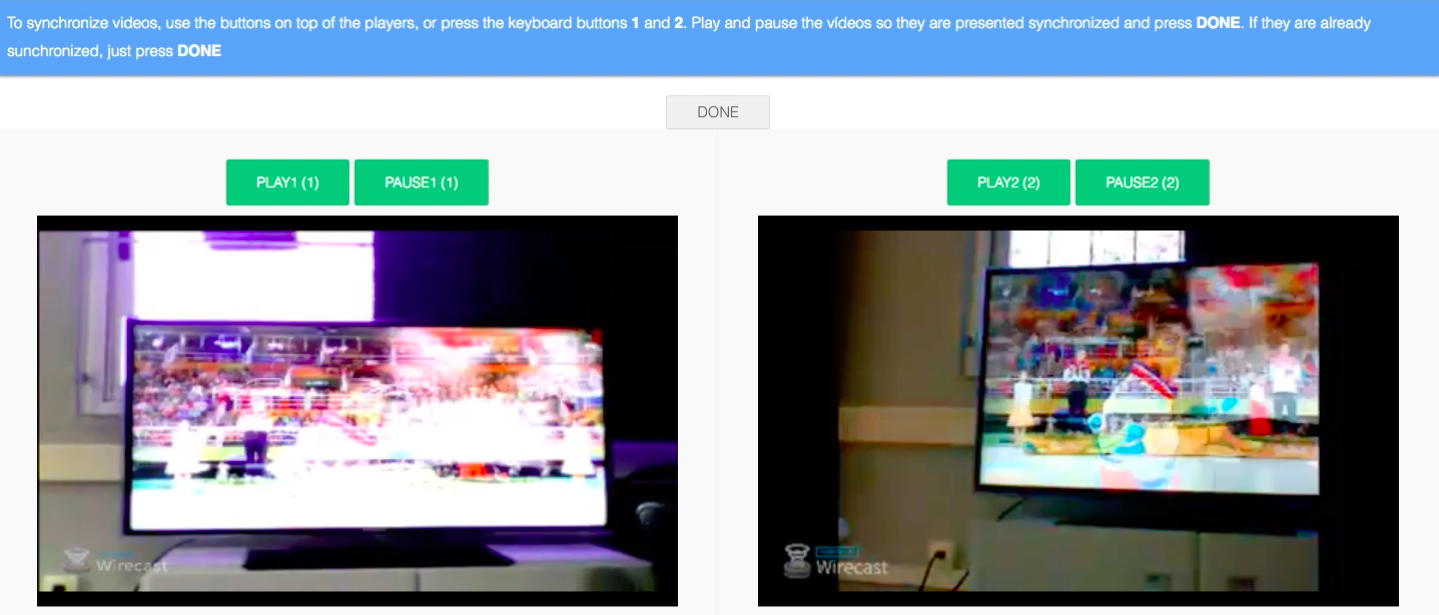
\includegraphics[scale=0.2] {figure/screen}}
	\caption{Live Streams from Olympic Games Synchronized through two different cameras}
	\label{live_tvs}
\end{figure}

On the top we have all information necessary to the user. He can aggregate new videos using the ADD NEW VIDEO options, SYNCHRONIZE the videos if he thinks the videos are not synchronized or he can just select the videos he want to watch. When just playing two selected videos from the videos list, each video player creates an instance for the player that is compatible with that source (YouTube or WebSocket). It is invisible to the user where the video is coming from.

When the user adds a video, an input text is shown to him, and he can add the video URI (WebSocket) or video ID (YouTube). The page reloads and the new video is listed in the video list for everyone that connects to the application. When the video is added by the user, an message is sent to the Coupler, containing the action to add a new asset to the DAL, and the specification of it, such as label and URI.

The last functionality of the MashUp is to synchronize the videos. When the user clicks on SYNCHRONIZE, a new mode of the application is revelled showing the synchronization tools. We use a Play 'n Pause approach to synchronize the videos. After the user thinks the videos are synchronized, clicking the DONE button, his contribution is sent to the Coupler and stored in the DAL for further processing of the relation.

\textbf{\textit{Play 'n Pause:}} If two videos with a certain degree of similarity, are presented to an individual from the crowd, he can possibly notice that one video is ahead of the other. This way, he can pause the video that is ahead on time while the other remains playing, until reaching a point of synchronization. Then, the user can resume playback of the first video. This process can be repeated until an individual feels like both videos are being presented synchronously. On \url{https://goo.gl/HTzecL}, readers can see the play and pause technique being used to synchronize two live streams from from Two YouTube servers.




%%%%%%%%%%%%%%%%%%%% ACM %%%%%%%%%%%%%%%%

%\textbf{\textit{MashUp Player}}

%Mashups are applications generated by combining content, presentation or other applications functionalities from disparate sources. They aim to combine these sources to create useful new applications or services (the offer and consumption of data between two devices) to users. In LiveSync we combine videos coming from different sources and platforms with the synchronization information from the coupler to reproduce a synchronous presentation of these videos.

%The MashUp Player (Figure~\ref{live_tvs}) is responsible for both presenting video synchronously and collecting the synchronization. Figure~\ref{live_tvs} represents the interface of the MashUp during a test: two cameras live streaming (content providers) a simulated television event to our mashup application.

%\begin{figure}[h]
%	\centerline{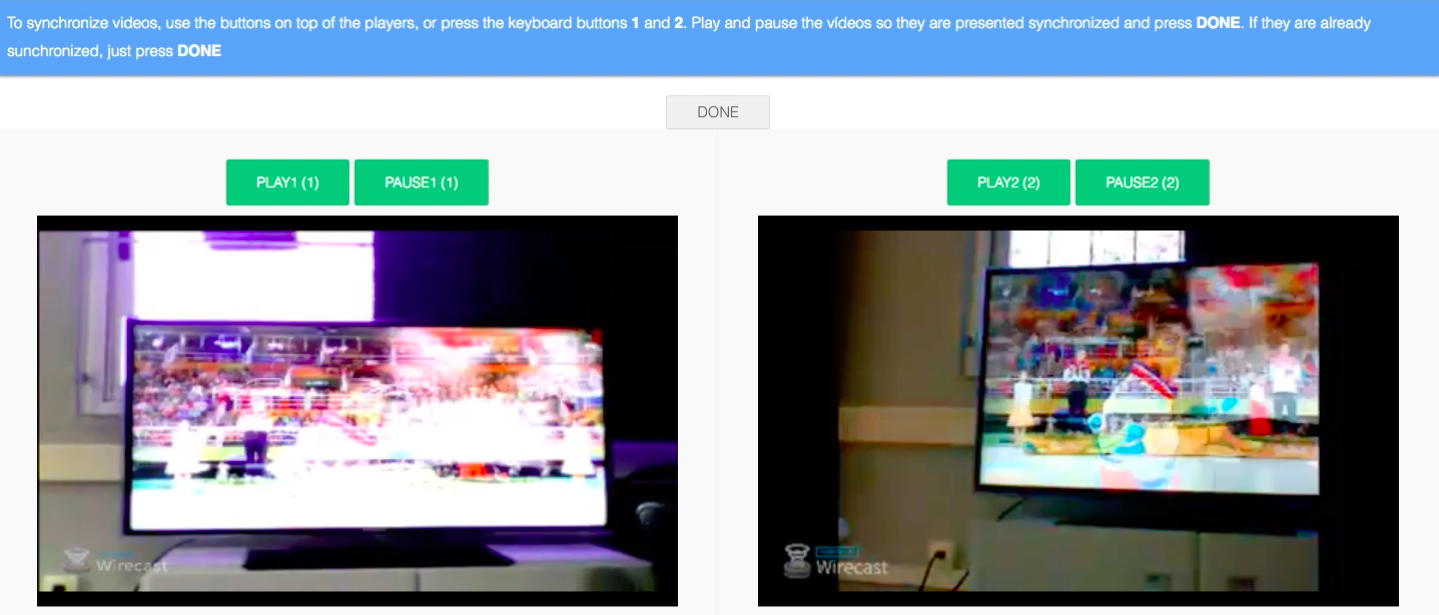
\includegraphics[scale=0.2] {figure/screen}}
%	\caption{Live Streams from Olympic Games Synchronized through two different cameras}
%	\label{live_tvs}
%\end{figure}

%On the top we have all information necessary to the user. He can aggregate new videos using the ADD NEW VIDEO options, SYNCHRONIZE the videos if he thinks the videos are not synchronized or he can just select the videos he want to watch. When just playing two selected videos from the videos list, each video player creates an instance for the player that is compatible with that source (YouTube or WebSocket). It is invisible to the user where the video is coming from.

%When the user adds a video, an input text is shown to him, and he can add the video URI (WebSocket) or video ID YouTube). The page reloads and the new video is listed in the video list for everyone that connects to the application. When the video is added by the user, an message is sent to the Coupler, containing the action to add a new asset to the DAL, and the specification of it, such as label and URI.

%The last functionality of the MashUp is to synchronize the videos. When the user clicks on SYNCHRONIZE, a new mode of the application is revelled showing the synchronization tools. We use a Play ’n Pause approach to synchronize the videos. After the user thinks the videos are synchronized, clicking the DONE button, his contribution is sent to the Coupler and stored in the DAL for further processing of the relation.